\begin{singlespacing}
\chapter{The \atlas\ Experiment}
\label{chapter:experiment}
%
\begin{epigraphs}
\qitem{%
if observing outer space gives us a view of the past, observing inner space
would surely give us a glimpse into the future - would be interesting if NASA
made a telescope for that%
}%
{Ken~M,
\textit{Comment: Yahoo! News},
2012~\cite{kenm2012inner}}
\end{epigraphs}
\end{singlespacing}
\noindent
Towards explaining the main result of this thesis,
a search for effects from supersymmetric models
in data from the \atlas\ detector
on the Large Hadron Collider (LHC)~\cite{
atlas2022searches,
atlas2008experiment,
lhc2008machine
},
we first cover some relevant facts about the design and motivations
behind \atlas.

The \atlas\ detector was not delivered in a preordained form.
It was designed with intent to provide maximally useful and novel data within
real-world cost budgets.
Within ambitions for general-purpose utility, \atlas's designs aimed to
construct a detector that could
\begin{itemize}
\item find the Higgs boson (which was predicted but yet unseen),
\item precisely measure known massive objects ($W$, $Z$, and $t$),
\item discover new (supersymmetric) particles~\cite{atlas1999design1}.
\end{itemize}
We now review these three goals with the subsequent news from \atlas's
operations.

\paragraph{Find the Higgs boson.}
Prior to \atlas's construction, the Higgs boson mass (and existence) was
poorly known, but loosely constrained by results like
$m(H) \gtrsim 90\,\eV[G]$ from searches at the
Large Electron–Positron Collider (LEP),
$m(H) = 76^{+85}_{-47}\,\eV[G]$ from other data on the electroweak sector,
and $m(H) \lesssim 1\,\eV[T]$ from theoretical unitarity arguments~\cite{
atlas1999design2,
ghinculov1998perturb,
lep1999ewk
}.

The Higgs boson couples to an extraordinary variety of fundamental particles.
For its discovery alone, \atlas's designers achieved sensitivity across the
entire $100$ to $1000\,\eV[G]$ window by targetting decays including
$h \to b\bar b$,
$h \to \gamma\gamma$,
$h \to ZZ^* \to 4\ell$, and
$h \to ZZ \to \ell\ell\nu\nu$;
these channels demand precise measurements of leptons, photons, and
$b$-jets (jets seeded from $b$ quarks), as well as sensitivity to the missing
transverse momentum of invisible neutrinos for $ZZ \to \ell\ell\nu\nu$ decays
at the very highest masses.

Both \atlas\ and \cms\ have now found a Higgs boson candidate at
$m(h) = 125\,\eV[G]$~\cite{
atlas2012higgs,
atlas2012combined,
cms2012higgs
}
and confirmed all of its tested Standard Model properties~\cite{
combined2016higgs,
atlas2022ten,
cms2022ten
}
such as its production mechanisms, decay rates,
spin, and parity~\cite{
HIGG-2013-01,
HIGG-2013-17,
HIGG-2014-06
}.

\paragraph{Precisely measure known massive objects.}
Other than the Higgs boson, the heavy Standard Model resonances are the
$W$ and $Z$ bosons and the top quark.
All of these are produced at high rates in LHC proton-proton collisions,
and present opportunities for \atlas\ to measure their properties
(such as masses and production cross-sections) with unprecedented precision.

Sensitivity to hadronic momenta is crucial,
both directly to measure heavy hadronic decays
(like $t \to bq\bar{q}$),
and indirectly for the missing transverse momenta from semi-invisible
leptonic decays (like $W \to \ell\nu$).
Since individual hadron identities are less relevant to these measurements,%
\footnote{%
Rare decays like
$W^\pm \to \pi^\pm \gamma$ or $W^\pm \to \pi^\pm \pi^+ \pi^-$
could give clean signals, but are not competitive due to their
tiny production rates and difficult identification~\cite{
cdf1996search,
mangano2014wpiy,
cms2021wpiy
}.
Leptonic $B$ hadron decays are useful in $m(t)$ measurements, but do not
require hadron identification~\cite{
CDF:2009mbf,
CMS:2016ixg,
ATLAS:2022jbw
}.%
}
it makes sense for \atlas's design to forfeit hadron identification systems
in favour of precise calorimetry with total angular coverage.

\atlas\ has now produced a plethora of competitively precise measurements
of the heavy Standard Model~\cite{atlas2021summarysm},
including $m(W)$~\cite{atlas2018wmass} and
$m(t)$~\cite{atlas2022symmarytop, atlas2019topmass, TOPQ-2015-03},
but also details of differential cross-sections~\cite{
STDM-2016-11,
STDM-2016-14,
TOPQ-2018-15,
TOPQ-2016-10
}.
Rare processes have also been studied in new levels of detail,
including
electroweak diboson ($WW/WZ/ZZ$ etc.)~\cite{
STDM-2015-21,
STDM-2015-23,
STDM-2017-09
}
and triboson~\cite{
STDM-2016-06,
STDM-2017-22,
STDM-2019-09
},
and rare top processes
($\ttbar Z$, $\ttbar W$ etc.)~\cite{
TOPQ-2013-05,
TOPQ-2018-01,
TOPQ-2020-03
},
These continue to not invalidate the Standard Model, and are aided in their
sensitivity by the lack of new phenomena,
which could have overpowered these rare signals.

\paragraph{Discover new (supersymmetric) particles.}
High-energy proton-proton collisions at the LHC therefore offer sensitivity
to new particles up to multi-$\eV[T]$ mass scales.
Heavy new particles are anticipated to either decay to known Standard Model
objects, or to be invisible in \atlas.
Designs that can discover such new particles are therefore neatly aligned with
our other goals of refining the current Standard Model
and to discovering the Higgs boson at any mass.
Visible decay products should already be caught by \atlas's abilities
to measure the Higgs boson and other Standard Model particles,
and the prospect of new invisible particles reinforces the need for precise
measurements of the missing transverse momentum.

Indeed, the main search presented in this thesis~\cite{atlas2022searches}
joins nicely with the pre-existing needs for sensitivity to signatures
including
$h \to b\bar b$
and
$ZZ \to \ell\ell\nu\nu$.

Dozens of searches for new phenomena have now been conducted in \atlas\ data,
with~\cite{
ATL-PHYS-PUB-2022-013
}
and without~\cite{
ATL-PHYS-PUB-2022-007,
ATL-PHYS-PUB-2022-012,
ATL-PHYS-PUB-2022-036,
ATL-PHYS-PUB-2022-034
} supersymmetry,
and show no convincing evidence for effects beyond the Standard Model.
This is not a failure. It is a success.
Our goal in science is not to discover something that is not there,
but to learn more about nature.
Finding no tangible new particles in LHC conditions is itself a discovery.


\section{Design}
Atlas is a Titan.
\atlas\ is the largest detector experiment at the LHC,
and alongside its biggest neighbours
\cms~\cite{cms2008experiment},
\lhcb~\cite{lhcb2008experiment},
and ALICE~\cite{alice2008experiment}
it is a multi-kilotonne beast,
and a wonder of scientific engineering~\cite{
atlas1994proposal,
atlas2008experiment,
atlas1999design1,
atlas1999design2
}.

Our search paper~\cite{atlas2022searches} contains concise and standard
descriptions of the \atlas\ detector and its relevant components.
Through its many inexact reproductions in past \atlas\ publications, the text
of these descriptions has become so highly refined that attempts to improve
it myself would probably be in vain.
Instead, this section quotes our published text with explanatory commentary.

\begin{figure}[tp]
\centering
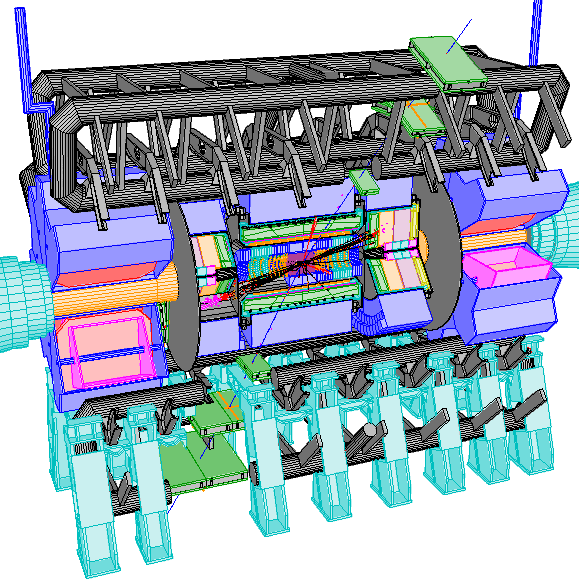
\includegraphics[width=0.6\textwidth]{figures/atlas_cutaway_volume_1.pdf}
\caption[
A central slice of \atlas's design
]{%
A central slice of \atlas's design, reproduced from~\cite{atlas1999design1,
persint2014manual},
including a simulated event that interacts with several sensitive subsystems.
}
\label{fig:atlas_cutaway}
\end{figure}

\begin{quote}
``%
The ATLAS detector~\cite{atlas2008experiment} is a multipurpose particle
detector with a forward--backward symmetric cylindrical geometry and a near
$4\pi$ coverage in solid angle.%
\footnote{%
``ATLAS uses a right-handed coordinate system with its origin at the nominal
interaction point (IP) in the centre of the detector and the $z$-axis along the
beam pipe.
The $x$-axis points from the IP to the centre of the LHC ring, and the $y$-axis
points upwards.
Cylindrical coordinates $(r,\phi)$ are used in the transverse plane, $\phi$
being the azimuthal angle around the $z$-axis.
The pseudorapidity is defined in terms of the polar angle $\theta$ as
$\eta = -\ln \tan(\theta/2)$.
Angular distance is measured in units of
$\Delta R \equiv \sqrt{(\Delta\eta)^{2} + (\Delta\phi)^{2}}$.%
''\footnotemark~\cite{atlas2022searches}%
}
It consists of an inner tracking detector surrounded by a thin superconducting
solenoid providing a $2\,\mathrm{T}$ axial magnetic field, electromagnetic and
hadronic calorimeters, and a muon spectrometer.%
''~\cite{atlas2022searches}
\end{quote}
To illustrate this description, a vertical slice of \atlas\ is displayed in
Figure~\ref{fig:atlas_cutaway}, and each subsystem is described in more detail
in a subsection below:
the inner tracking detector in Section~\ref{sec:atlas_inner},
the electromagnetic and hadronic calorimeter systems in
Section~\ref{sec:atlas_calo},
and
the chambers of the muon spectrometer in Section~\ref{sec:atlas_muon}.
The final connection to the data analysed in this thesis is made through the
trigger system which is described in Section~\ref{sec:atlas_trigger},
and details of the data themselves are given in
Section~\ref{sec:atlas_data}

\footnotetext{%
This footnote appears in every \atlas\ publication, but was perfected
in~\cite{lester2013heffalon}.
True to form, internal \atlas\ guidelines ask that
``If you think you can improve on it, please consult with the
Publications Committee''~\cite{atlas_coordinate, atlas_footnote}.
}


\section{Inner detector}
\label{sec:atlas_inner}
The inner tracking detectors begin \atlas's measurements of new collisions
by precisely tracing the paths taken by energetic charged particles
as they curve through the solenoidal magnetic field.
Track curvature provides momentum information,
tracks' associations into collision vertices helps to separate the multiple
scatterings per crossing (pile-up),
and their associations into displaced vertices help to identify
decays.
\begin{quote}
``%
The inner tracking detector covers the pseudorapidity range $|\eta| < 2.5$.
It consists of silicon pixel, silicon microstrip, and transition radiation
tracking detectors.
An additional layer of silicon pixels, the insertable
B-layer~\cite{ATLAS-TDR-19, PIX-2018-001}, was installed before Run~2.%
''~\cite{atlas2022searches}
\end{quote}
This insertable B-layer is a silicon pixel detector that begins just
$3\,\textrm{cm}$ from the beam-pipe, and provides robust tracking for the
present and future high LHC luminosities,
particularly for sensitivity to particles whose lifetimes are just right to
decay inside the tracking system;
these `Goldilocks Zone' particles include B-hadrons, some tau leptons, and
maybe new species.

Following radially outwards, the silicon pixel and silicon microstrip%
\footnote{%
Formerly known as the SemiConductor Tracker~\cite{atlas1999design1},
the silicon microstrip system retains the acronym
SCT~\cite{atlas2008experiment}.%
}
detectors (which use silicon technology)
and the transition radiation tracking detectors (which uses `straw' tubes
gas tubes).

As for the whole \atlas\ detector, complete $\phi$ coverage and a large $\eta$
range minimizes leakage.
Towards \atlas's design goals, this inner tracking detector crucially provides
measurements of electrons, B-hadrons, and contributes to the reconstruction of
missing transverse momentum.


\section{Calorimeters}
\label{sec:atlas_calo}
Inelastic collisions cause energetic particles to scatter, distributing their
energy into macroscopic particle showers.
Calorimetry uses this principle to measure energies
by interleaving dense absorbing materials (which initiate showers)
with sensitive materials that convert showers into electrical signals.
In \atlas,
\begin{quote}
``%
Lead/liquid-argon (LAr) sampling calorimeters provide electromagnetic (EM)
energy measurements with high granularity.
A steel/scintillator-tile hadron calorimeter covers the central pseudorapidity
range ($|\eta| < 1.7$).
The end-cap and forward regions are instrumented with LAr calorimeters for both
the EM and hadronic energy measurements up to $|\eta| = 4.9$.%
''~\cite{atlas2022searches}
\end{quote}
The electromagnetic calorimeters provide located electron/photon energy
measurements,
and the hadronic calorimeters subsequently aim to stop and measure hadronic
activity for later analysis in jet clustering.
Maximal angular coverage by the calorimeters further facilitates missing
transverse momentum estimates.

Neither `A' in \atlas\ stands for Argon, but perhaps one should.
Liquid-argon is the chosen active material in the electromagnetic and forward
calorimeters for its robust, linear response in converting showers to
electrical signals for readout by electrodes.
Liquid argon is poured as a liquid to fill the gaps between the various
metallic absorbers, which are folded into zigzag ``accordion'' shapes that
optimize uniformity around the detector.
The steel/scintillator hadronic tile calorimeter is a
``simple and cost effective''~\cite{atlas1996tile} design, which uses
photomultiplier tubes to convert light from its polystyrene scintillators into
electrical signals.
Particles lose some energy before reaching the calorimeters; a thin
liquid-argon pre-sampler is installed before the central EM calorimeter
to regain such loss.

These calorimeter systems achieve attenuations of at least ten interaction
lengths throughout their $|\eta| < 4.9$ range;
by maximizing this attenuation, the design minimizes noise from hadronic
`punch-through' of non-muons into the muon system.


\section{Muon system}
\label{sec:atlas_muon}
Muons penetrate matter well because of their large mass and non-interaction
with the strong nuclear force.
\atlas\ doesn't try to stop energetic muons;
above around $3\,\eV[G]$, they pass right through the calorimeters, and are
instead measured by their curved tracks in a toroidal magnetic field that
envelopes dedicated detectors on \atlas's periphery.
\begin{quote}
``%
The muon spectrometer surrounds the calorimeters and is based on three large
superconducting air-core toroidal magnets with eight coils each.
The field integral of the toroids ranges between $2.0$ and
$6.0\,\mathrm{T\kern-0.15ex m}$ across most of the detector.
The muon spectrometer includes a system of precision chambers for tracking and
fast detectors for triggering.%
''~\cite{atlas2022searches}
\end{quote}
Muon subsystems come in four varieties, all of which operate by detecting
charges scattered by the muons as they fly through gaseous media.
Together, these systems track the muons' paths as the magnets bend them in the
longitudinal plane; these toroidal magnets generate fields outside the tile
calorimeter around the central barrel and in the end-caps as illustrated in
Figure~\ref{fig:atlas_magnets}.

\begin{figure}[tp]
\centering
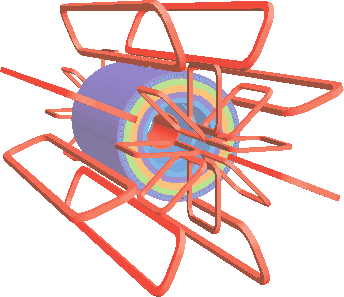
\includegraphics[width=0.6\textwidth]{figures/atlas_magnets.pdf}
\caption[
Layout of \atlas's toroidal magnets around the tile calorimeter and inner
solenoid
]{%
Layout of \atlas's toroidal magnets around the tile calorimeter and inner
solenoid, including the eight barrel and end-cap coils,
reproduced from~\cite{atlas2008experiment}.
The \atlas\ muon spectrometer measures muons' tracks as they bend through
this peripheral magnetic field.
}
\label{fig:atlas_magnets}
\end{figure}

Measurements of the tracks' curvature yield estimates of the muons' momenta;
although extremely energetic muons will have straight tracks,
\atlas's construction and calibration achieves a high precision, which
increases to only $10\%$ relative error on tracks with $1\,\eV[T]$ transverse
momenta~\cite{
atlas1994proposal,
atlas2008experiment,
ATL-PHYS-PUB-2015-037
}.


\section{Trigger}
\label{sec:atlas_trigger}
The LHC's $25\,\mathrm{ns}$ time difference between proton bunches
(bunch spacing) is so fast that light-speed particles ejected from one crossing
are still zipping through \atlas's $12.5\,\textrm{m}$ radius when the next
collision arrives.
This extreme engineering is necessary to achieve the integrated luminosities we
need to see rare effects, but to avoid becoming overwhelmed
by data it also demands a strict data reduction mechanism.
This mechanism is the trigger:
\begin{quote}
``%
A two-level trigger system is used to select events.
The first-level trigger is implemented in hardware and uses a subset of the
detector information to accept events at a rate below $100\,\mathrm{kHz}$.
This is followed by a software-based trigger that reduces the accepted event
rate to $1\,\mathrm{kHz}$ on average depending on the data-taking conditions.%
''~\cite{atlas2022searches}
\end{quote}
The first-level (L1) trigger uses its fast preliminary information to accept
interesting event and mark their regions of interest.
Complete data in these regions of interest are passed to the second-level
(high-level trigger, HLT) to inform its decision of whether to accept each
event.
Events accepted by the HLT are recorded for future analysis~\cite{
atlas2016trigger,
atlas2008experiment
}.


\section{Data}
\label{sec:atlas_data}
Raw binary data are hard for us humans to interpret.
Before use in publishable analysis projects, software systems first mutate
those data into a workable form, of clean events with calibrated and
interpretable event variables.
\begin{quote}
``%
An extensive software suite~\cite{ATL-SOFT-PUB-2021-001} is used in the
reconstruction and analysis of real and simulated data, in detector operations,
and in the trigger and data acquisition systems of the experiment.%
''~\cite{atlas2022searches}
\end{quote}
Prediction is important in data analysis.
This software suite helps to generate predictive simulations, and provides
realism by passing both the real and simulated data through the same processing
pipelines~\cite{SOFT-2010-01, geant2003}.
Software models of the \atlas\ detector itself are refined with the results from
many calibration studies and in-situ measurements~\cite{atlas2008experiment},

The search presented in this thesis uses data from proton-proton collisions at
$\sqrt{s} = 13\,\eV[T]$ centre-of-mass energies in Run~2 of the
LHC, in which \atlas\ collected data in the years
$2015\textrm{--}2018$~\cite{atlas2022searches}.
This second run has various refinements over the Run~1, including beam energies
increasing from $\sqrt{s} = 7\textrm{ or }8\,\eV[T]$, and bunch spacings
halving from $50$ to $25\,\textrm{ns}$~\cite{lhc2006run2}.

Data collected under anomalous detector operations are hard to model.
Lists are maintained indicating which datasets arise from `good', normal
detector operations, and these lists are commonly employed to select only clean
subsets of good data for analysis projects.
Testament to the quality of \atlas's operations, this cleaning removes less
than $5\%$ of the Run~2 data~\cite{
DAPR-2018-01,
Golling:2011zy
}.

% closing comment?
Now that we have predictive models, in the Standard Model and supersymmetric
alternatives,
and interpretable data, from \atlas's measurements of LHC collisions,
we are ready to begin to squeeze some useful research from those data.

% this comment activates enlarged spacing for the final paragraph lol
